  \documentclass[a4paper, 11pt, titlepage]{article}
\usepackage[a4paper,top=2.25cm,bottom=2.25cm,left=2cm,right=2cm,marginparwidth=2cm]{geometry}
\usepackage{amsmath}
\usepackage{graphicx}
\usepackage[toc,page]{appendix}
\usepackage[colorlinks=true, allcolors=blue]{hyperref}
\usepackage{caption}
\usepackage{titlepic}
\usepackage{titling}
\usepackage{wrapfig}
\usepackage{stfloats}
\usepackage{placeins}
\usepackage[urldate=iso,seconds=true]{biblatex} %Imports biblatex package
\addbibresource{sample.bib} %Import the bibliography file
\usepackage[english,serbian]{babel}
\usepackage{framed}
\usepackage[dvipsnames]{xcolor}
\usepackage{tcolorbox}
\usepackage{listings}
\usepackage{xcolor}

\definecolor{codegreen}{rgb}{0,0.6,0}
\definecolor{codegray}{rgb}{0.5,0.5,0.5}
\definecolor{codepurple}{rgb}{0.58,0,0.82}
\definecolor{backcolour}{rgb}{0.95,0.95,0.92}

\lstdefinestyle{mystyle}{
    backgroundcolor=\color{backcolour},   
    commentstyle=\color{codegreen},
    keywordstyle=\color{magenta},
    numberstyle=\tiny\color{codegray},
    stringstyle=\color{codepurple},
    basicstyle=\ttfamily\footnotesize,
    breakatwhitespace=false,         
    breaklines=true,                 
    captionpos=b,                    
    keepspaces=true,                 
    numbers=left,                    
    numbersep=5pt,                  
    showspaces=false,                
    showstringspaces=false,
    showtabs=false,                  
    tabsize=2
}

\lstset{style=mystyle}

\def\departman{Departman za računarstvo i automatiku}
\def\odsek{Odsek za računarsku tehniku i računarske komunikacije}
\def\reporttitle{Software PWM over busy wait} 
\def\institutionname{UNIVERZITET U NOVOM SADU}
\def\institutionnames{FAKULTET TEHNIČKIH NAUKA}
\def\cityname{NOVI SAD}
\def\authornameA{Kandidat: Aleksandar Ćetković RA 24/2021} 
\def\authornameB{Kandidat: Vuk Antović RA 52/2021} 
\def\authornameC{Kandidat: Ana Mujić RA 58/2021} 
\def\authornameD{Kandidat: Stefan Mitić RA 216/2021} 
\def\predmet{Predmet: Operativni sistemi u realnom vremenu}
\def\mentor{Mentor rada: dr Miloš Subotić}
\title{\reporttitle}
\def\reportsubtitle{PROJEKTNI ZADATAK}
\date{\today}

\usepackage{fancyhdr}
\pagestyle{fancy}
\fancyhf{}
\lhead{\reporttitle}
\setlength{\headheight}{13.6pt}
\addtolength{\topmargin}{-1.6pt}
\rfoot{\thepage}

\begin{document}
\begin{titlepage} 
\newcommand{\HRule}{\rule{\linewidth}{0.5mm}}

\center
\textsc{\Large \institutionname}\\[0.2cm]
\textsc{\Large \institutionnames}\\[0.2cm]
\textsc{\Large \cityname}\\[0.2cm]
\textmd{\Large \departman}\\[0.1cm] 
\textmd{\Large \odsek}\\[0.1cm] 


\HRule\\[0.8cm]

{\huge\bfseries \reporttitle}\\[0.4cm]
\ifx\reportsubtitle\undefined 
\else
    {\textsc{\Large \reportsubtitle}}\\[0.4cm] 
\fi

\HRule\\[1.5cm]


\authornameA \\[0.5cm]
\authornameB \\[0.5cm]
\authornameC \\[0.5cm]
\authornameD \\[0.5cm]
\predmet\\[0.5cm]
\mentor \\[0.5cm]

\vfill\vfill\vfill\vfill\vfill\vfill\vfill\vfill\vfill\vfill\vfill\vfill\vfill\vfill\vfill\vfill\vfill\vfill\vfill\vfill\vfill

{\large Novi Sad, decembar, 2023.}

%\includegraphics[width=0.2\textwidth]{images/qut-logo.jpg}\\[1cm] % Include a department/university logo - this will require the graphicx package
 
\end{titlepage}
% \maketitle
{\hypersetup{linkcolor=black} 
% \let\clearpage\relax 
\thispagestyle{empty}
\newpage
\thispagestyle{empty}
\tableofcontents
\newpage
\
\pagenumbering{arabic}
}



\section{Uvod}
\rhead{Uvod}

\subsection{Opis problema}

Naš zadatak se svodi da napravimo softversko rešenje za tvrdi operativni sistem u realnom vremenu. 
Konkretnije, naši zadaci su: 
\begin{itemize}
  \item Logovanje PWM signala i vremenskih oznaka događaja
  \item Forsiranje operativnog sistema da u slučaju da ne stiže da završi izvršavanje datog događaja na vreme, da isti ne započinje.
  \item Iscrtavanje PWM signala, kašnjenja i distribucije kašnjenja pomoću skripte u Juliji

\end{itemize}


\subsection{Teorijske osnove}

Da bismo mogli da uspešno uradimo projekat, prvo moramo da razumemo neke osnovne pojmove i šta se zapravo dešava "ispod haube". 
\\

Prvo krećemo od pojma tvrdi operativni sistem u realnom vremenu, odnosno \textit{hard real time operative system}. 

Operativni sistemi u realnom vremenu postavljaju određene vremenske rokove do kad je potrebno da se neki zadatak uradi. U zavisnosti od načina rukovanja zadacima u slučaju kašnjenja, operativne sisteme u realnom vremenu možemo podeliti na "tvrde" (\textit{hard real time}) i "meke" (\textit{soft real time}). 
Tvrdi operativni sistem u realnom vremenu ne dopušta kašnjenje i u slučaju da zna da neki zadatak neće stići da se završi, on ga neće ni započeti. 
Meki operativni sistem u realnom vremenu dopušta određeno kašnjenje i dopušta početak zadataka koji se potencijalno neće završiti na vreme. 

\\

Mi ćemo se baviti \textit{hard real time} operativnim sistemom i implementirati rukovanje zadacima u slučaju njihovog kašnjenja. 
\\

Da bismo to uradili, potrebno je takođe da razumemo šta je PWM signal. 
\\
PWM (\textit{Pulse Width Modulation}) odnosno širinsko-impulsna modulacija jeste tehnika dobijanja analognih vrednosti pomoću digitalnih impulsa konstantne amplitude. Radi jednostavnosti, u nastavku teksta ćemo koristiti isključivo pojam PWM. 

Uz pomoć PWM signala, mi kontrolišemo hardver koji se pomera na određeni način (ugao pomeraja i slično). 

\subsection{Analiza problema}

Problem smo podelili na tri dela. 
\\

Prvo,logujemo vremenske oznake (\textit{timestamps}) da bismo mogli da ispratimo vremena zadataka i da li kasne. 
\\

Dalje, ograničavamo operativni sistem da ignoriše svaki zadatak čiji početak kasni i svaki zadatak čiji bi završetak bio nakon roka. 
\\

I na kraju potrebno je prikazati na grafiku sve vremenske oznake kada se sve implementira. 


\newpage
\section{Rešenje problema}
\rhead{Rešenje problema}

Rešenje ćemo prikazati u tri etape, koje su navedene u analizi problema.

Poenta zadatka jeste da sprečimo izvršavanje bilo kakvih zadataka koji kasne sa početkom ili završetkom.  \\

Da bismo to postigli, potrebno je prvo da ispišemo vremenske oznake događaja, odnosno zadataka. Zatim je potrebno da implementiramo same "blokade" koje sprečavaju da se događaj desi ako ne može da se izvrši do kraja do zadatog roka, a da bismo proverili da li sve to radi i da bismo lakše otklonili potencijalne greške, potrebno je da izvršimo vizuelizaciju vremenskih oznaka i događaja.  \\

Sve relevantne informacije (vremenske oznake, stanja, da li kasni ili ne, koliko kasni ako dođe do kašnjenja...) možemo prikazati uz pomoć grafika u okviru \textit{Plots} paketa u Juliji. 
\subsection{Logovanje vremenskih oznaka PWM signala}
Da bismo uopšte mogli da upisujemo vremenske oznake u fajl, pre svega moramo da inicijalizujemo logovanje pozivom funkcije \textit{log\_\_init} u funkciji \textit{main} datoteke \textit{main.c}. \\

Funkcija nema argumente, povratna vrednost joj je samo potvrda uspešnosti (0, 1 ili -1). \\

U \textit{log\_\_init} pravi se fajl u koji će se upisati vremenske oznake. \\ 

Dalje, u funkciji \textit{busy\_pwm\_loop} u datoteci \textit{busy\_pwm.c} u kojoj se vrti petlja i određuje vremena promene stanja PWM signala, pozivamo funkciju \textit{log\_\_add} koja doda razliku vremena buđenja niti i zadatog vremena u log fajl.  U log fajlu imamo i da li je vrednost PWM 1 ili 0 i imamo podatak sa kog kanala se upisuje. \\

  
\subsection{Hard Real Time}

U fajlu \textit{sw\_pwm.c} u funkciji \textit{busy\_pwm\_loop} imamo beskonačnu petlju koja obrađuje događaje. Tu je bitan dodatak uslov ukoliko je vreme događaja, odnosno krajnji rok izvršavanja događaja, manje od trenutnog vremena (na primer rok događaja je 700ms od početka programa a trenutno vreme je 1000 ms) onda ignorišemo taj događaj i prelazimo na sledeći jer smo zakasnili. \\ 

Ukoliko događaj zakasni, nit se uspava i čeka do roka sledećeg događaja.  



\newpage
\subsection{Vizuelizacija pwm signala u Juliji}

Pre svega, možemo prikazati kako izgleda PWM signal i njegova rastuća ivica. 

    \begin{figure}[h]
    \centering
    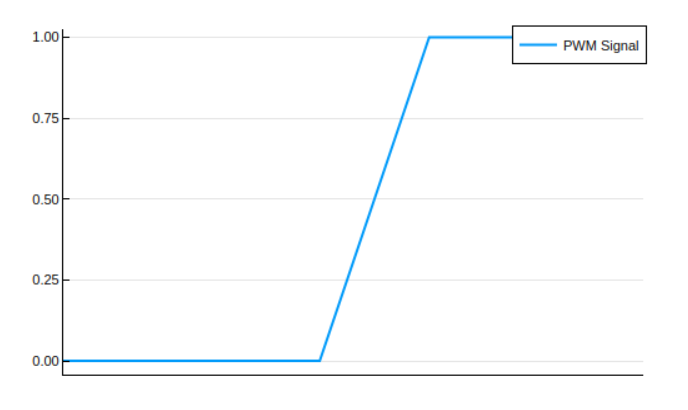
\includegraphics[width=0.50\linewidth]{rising_edge.png}
    \caption{Rastuća ivica PWM signala}
\end{figure}

\begin{figure}[h]
    \centering
    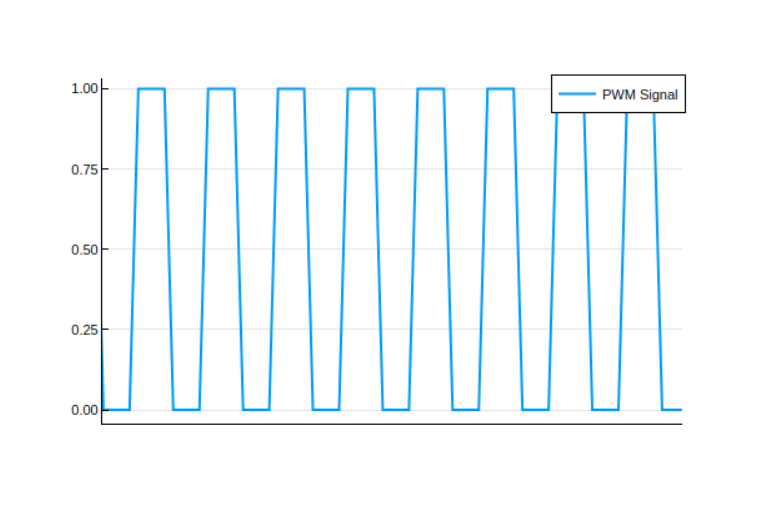
\includegraphics[width=0.50\linewidth]{PWM.png}
    \caption{PWM signal, ispune 50}
    
\end{figure}


Da bismo od datoteke koja sadrži vremenske oznake dobili nešto čitljivo, potrebno je u Juliji otvoriti fajl i parsirati liniju po liniju. \\

Koristimo tri niza, jedan za vremenske oznake kašnjenja, jedan za stanja signala (0 ili 1) i jedan za pin za koji je opisan događaj. \\

U svakoj liniji odvajamo podatak u odgovarajuć niz i plotovaćemo isključivo kašnjenje da bismo videli kašnjenja kroz vreme i statistički obradili.\\

Na kraju plotujemo kašnjenje, i vršimo aproksimaciju krive distribucije kašnjenja. \\
\begin{figure}
    \centering
    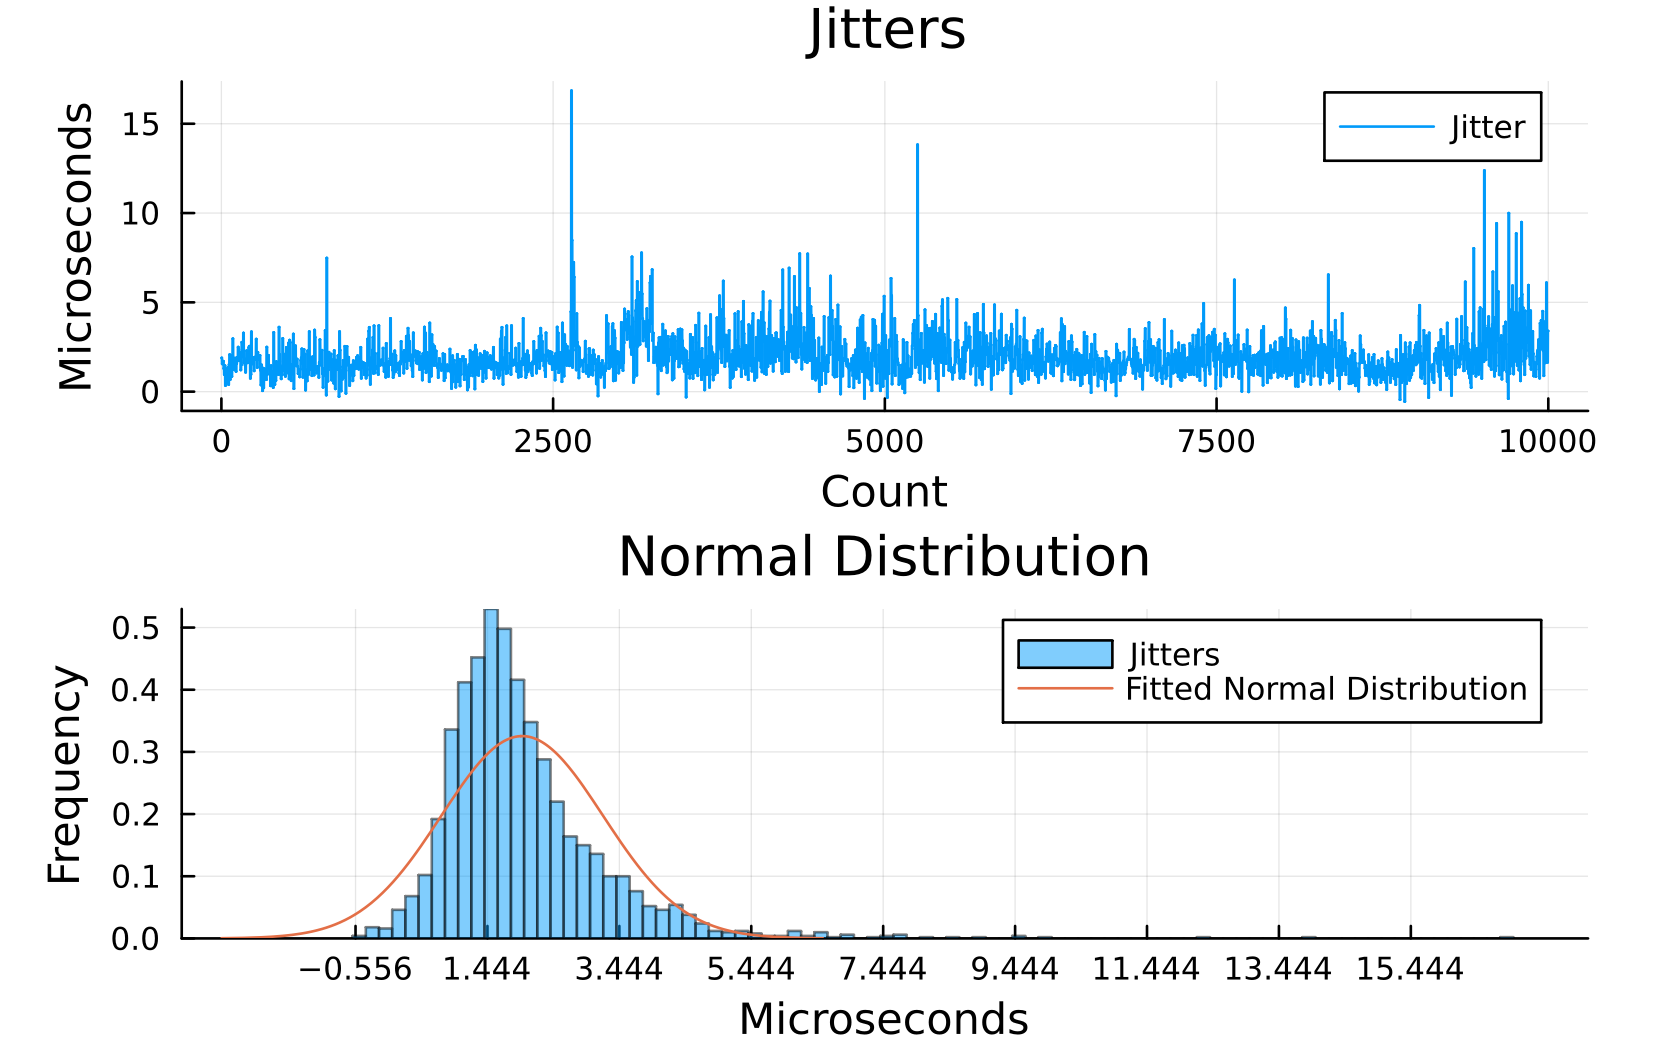
\includegraphics[width=1\linewidth]{dvagrafika.png}
    \caption{Grafici kašnjenja i distribucije}
\end{figure}
\newpage
\section{Pokretanje rešenja}
\rhead{Pokretanje rešenja}

Potrebno je navigirati se u folder $SW/Driver/motor\_ctrl$ i u terminalu ukucati komande: 

\begin{lstlisting}[language=bash, caption= Pokretanje programa]
sudo make 

sudo make start
\end{lstlisting}

Dalje, da bi se pokrenula skripta za iscrtavanje, potrebno je navigirati se u folder $SW/Scripts$ i u pokrenuti Juliu. Za pokretanje skripte koja radi u realnom vremenu: 
\begin{lstlisting}[language=bash, caption= Pokrtanje Julia skripte za grafik kašnjenja]
include("plot_real_time.jl")
\end{lstlisting}
A za pokretanje skripte koja se ne menja kroz vreme:
\begin{lstlisting}[language=bash, caption= Pokrtanje Julia skripte za iscrtavanje distribucije kašnjenja]
include("plot.jl")
\end{lstlisting}
\newpage
\section{Zaključak i završna reč}
\rhead{Zaključak i završna reč}

Za kraj, ceo proces projekta je iziskivao mnogo više vremena razmišljajući o načinu rada i implementiranju algoritma nego samoj implementaciji. \\

Korisni linkovi:  \\

\begin{itemize}
  \item GitHub repozitorijum: \url{https://github.com/OSSuRV-PWM-Busy-wait/OSuRV_2023/tree/main/PWM/SW} 
  \item YouTube link: \url{https://youtu.be/mqTBjuDcG8A}

\end{itemize}
\end{document}